\documentclass[12pt,a4paper]{scrartcl}
\usepackage[utf8]{inputenc}
\usepackage[ngerman]{babel}
\usepackage{amsmath,amssymb,amstext}
\usepackage{fancyhdr}
\usepackage{trsym,trfsigns}
\usepackage{graphicx}
\title{Integraltransformation}
\subtitle{Zusammenfassung}
\author{Grasso Antonino}
\date{Sommersemester 21}

\pagestyle{fancy}
\fancyhf{}
% Header
\lhead{Integraltransformation}
\rhead{Zusammenfassung}
% Footer
\cfoot{Grasso}
\rfoot{\thepage}

\begin{document}

% Title
\begin{titlepage}
\maketitle
\vspace{100px}

\end{titlepage}

% Table of contents
\tableofcontents
\newpage

% Content

\section{Verlauf und Rahmen}
\label{sec:verlauf-und-rahmen}
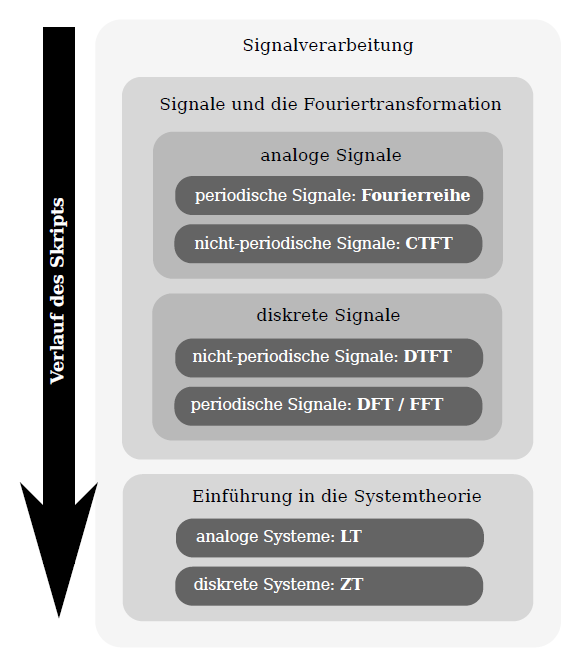
\includegraphics[height=10cm]{Pictures/Verlauf.png}

\section{Klassifizierung der Signale}
\label{sec:klassifizierung}
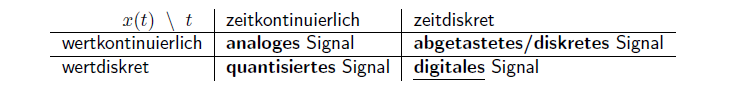
\includegraphics[height=2cm]{Pictures/Einheiten.png}

\section{Definitionen und Konstanten}
\label{sec:definitionen-und-konstanten}
\subsection{Periodendauer $T_p$}
\label{sec:sub:periodendauer}
$$ x(t) := \mathbb{R} \to \mathbb{R}$$
$$T_p := x(t + n \cdot T_p) = x(t)$$
\subsection{Frequenz $f$}
\label{sec:sub:frequenz}
$$f = \frac{1}{T_p} = \frac{\omega_p}{2\pi}$$
\subsection{Kreisfrequenz $\omega_p$}
\label{sec:sub:kreisfrequenz}
$$\omega_p = \frac{2\pi}{T_p}$$
\subsection{sinc-Funktion $sinc(t)$}
\label{sec:sub:sinc}
$$sinc(t) = \frac{\sin(t)}{t}$$
\subsection{Sprungfunktion $\varepsilon(t)$}
\label{sec:sub:sprungfunktion}
$$\varepsilon(t) := $$ 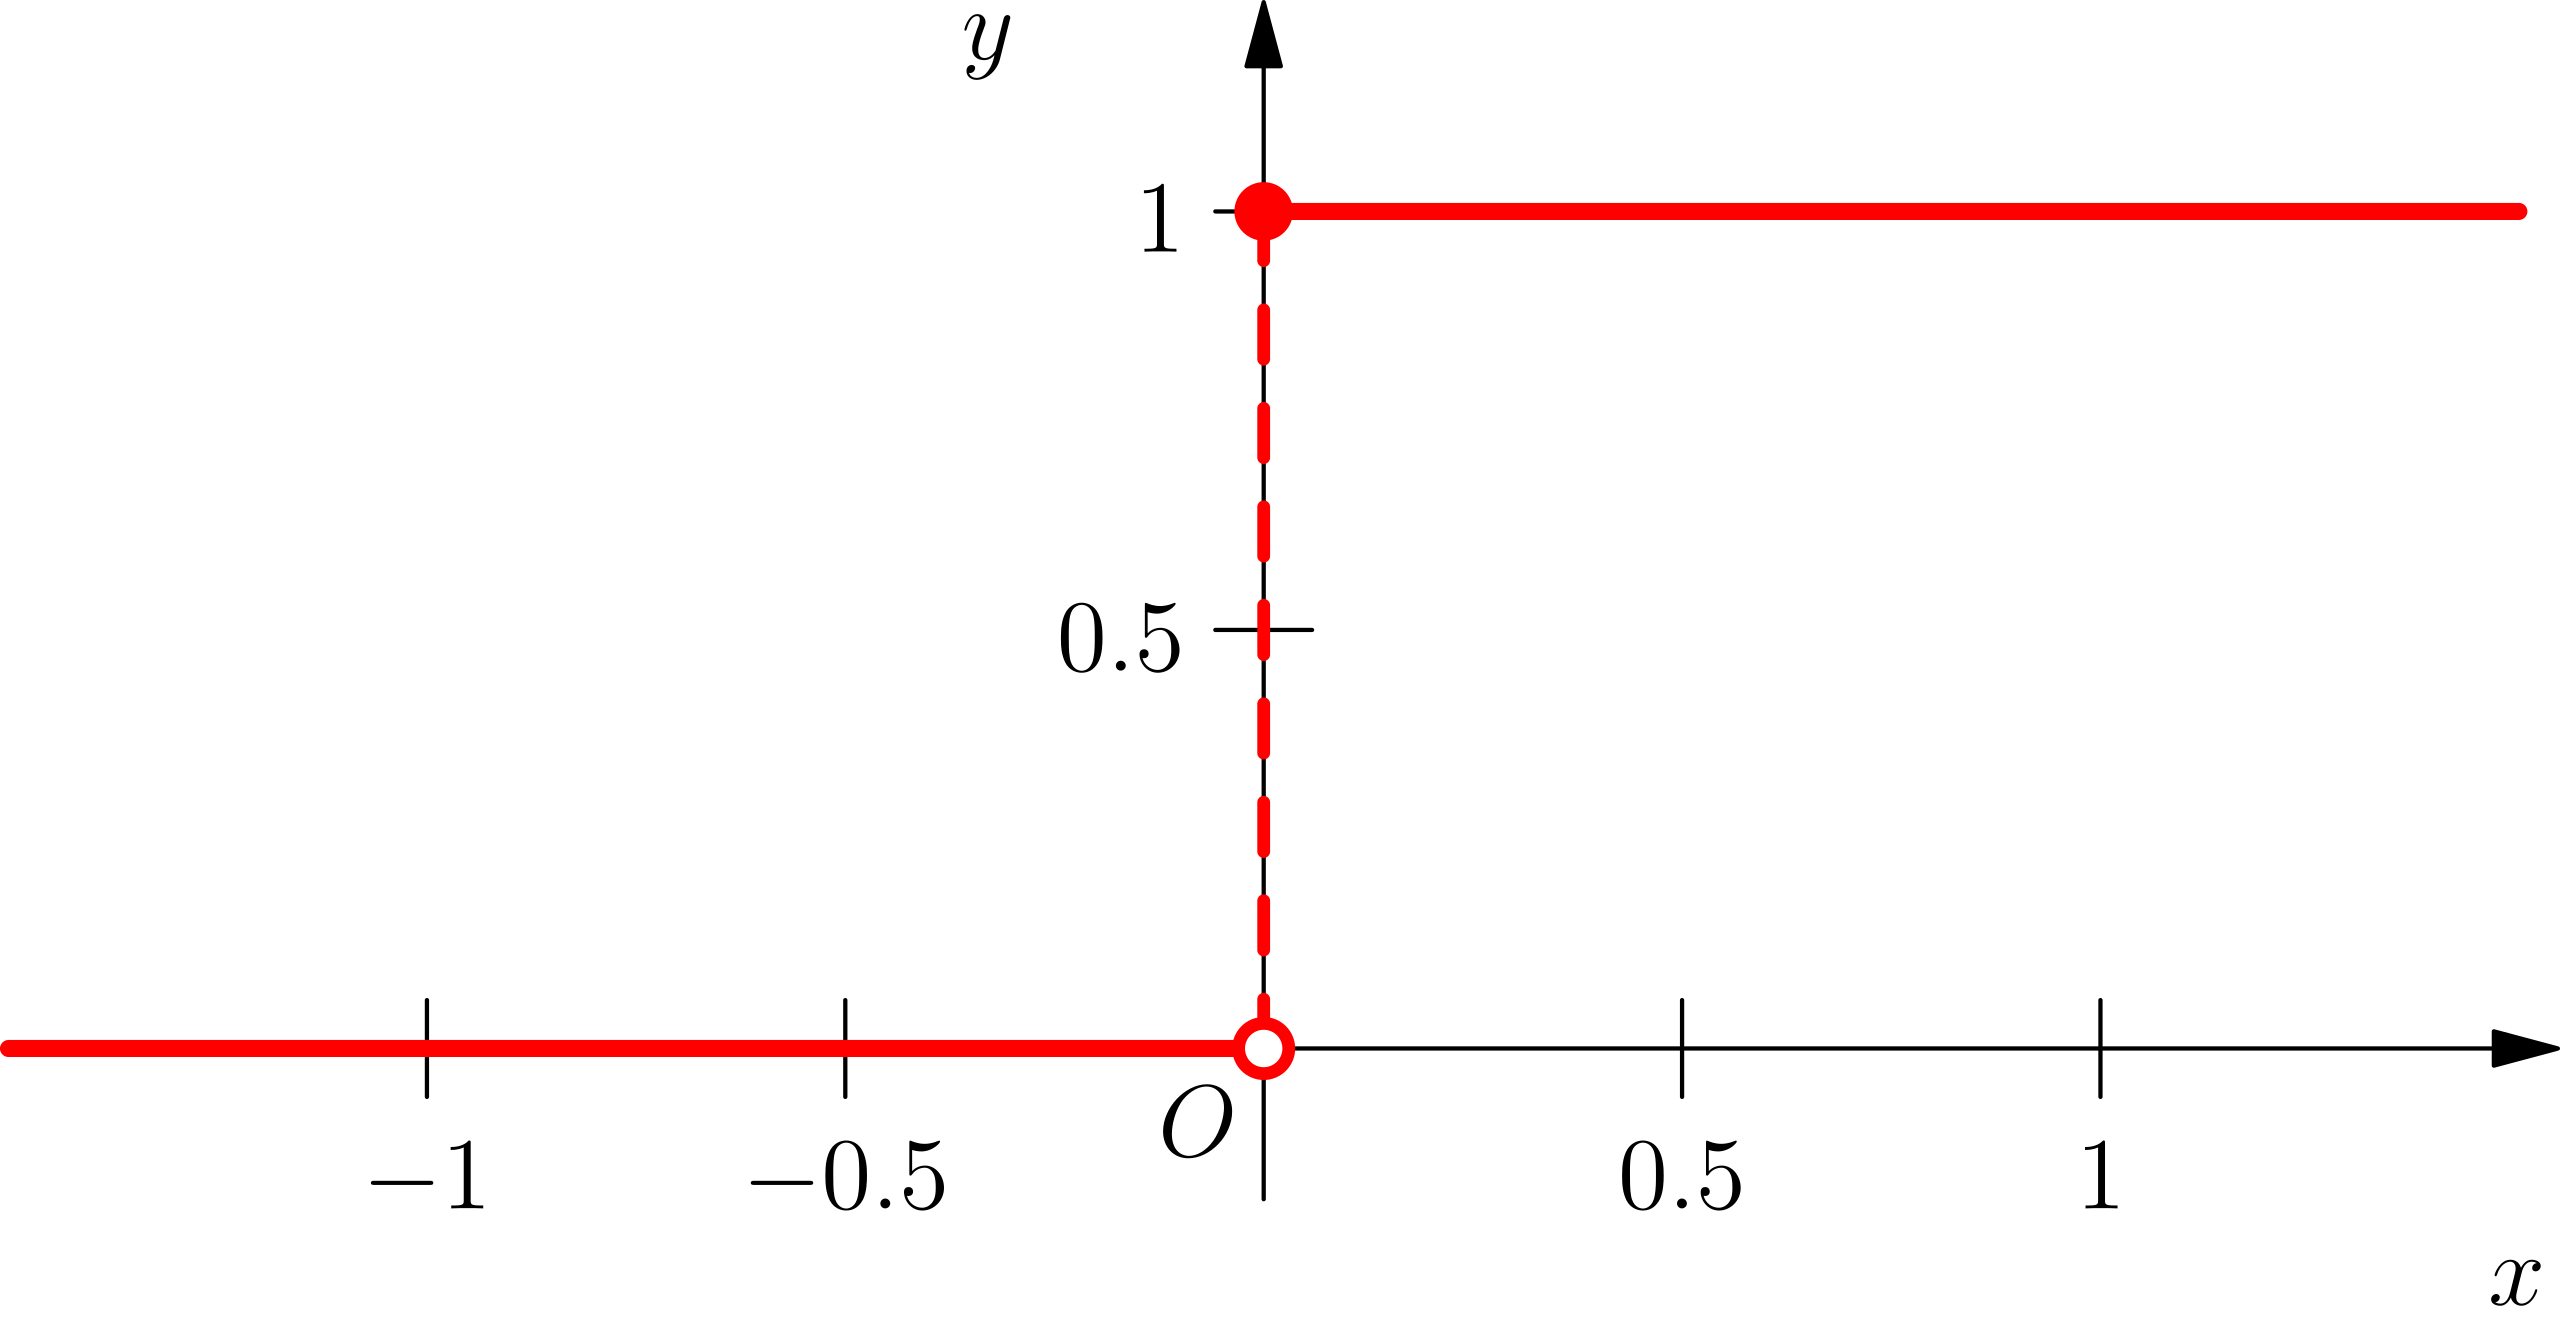
\includegraphics[height=5cm]{Pictures/Heaviside.svg.png}
\subsection{Zeitsignal $x(t)$}
\label{sec:sub:zeitsignal}
$$x(t) := Zeitsignal$$
\subsection{Frequenzspektrum $X(\omega)$}
\label{sec:sub:frequenzspektrum}
$$X(\omega) := Frequenzspektrum $$
\subsection{Abtastfrequenz $f_A$}
\label{sec:sub:abtastfrequenz}
$$f_A = \frac{1}{\Delta T_A} = \frac{\omega_p}{2\pi}$$
\subsection{Abgetastetes Zeitsignal $x_A(t)$}
\label{sec:sub:abgetastetes-zeitsignal}
$$x_A(t) := abgetastetes\ Zeitsignal$$
\subsection{Abgetastetes Frequenzspektrum $X_A(\omega)$}
\label{sec:sub:abgetastetes-frequenzspektrum}
$$X_A(\omega) := abgetastetes\ Frequenzspektrum $$
\subsection{Zeitspanne zwischen Abtastugnen }
\label{sec:sub:zeitspanne-zwischen-abtastungen}
$$\Delta T_A := Zeitspanne\ zwischen\ Abtastungen $$

\newpage
\section{Signale und Fouriertransformation}
\label{sec:signale-und-fouriertransformation}

\subsection{Analoge Signale}
\label{sec:sub:analoge-signale}

\subsubsection{Fourierreihe (analoge, periodische Signale)}
\label{sec:sub:sub:fourier-reihe}

Jedes Signal $x(t)$ kann als unendliche Summe von überlagerten Sinus und Cosinus Funktionen dargstellt werden: \\

\noindent  \textbf{Sinus-Cosinus-Darstellung der Fourierreihe:}
\begin{equation}
  \label{eq:1}
  \begin{split}
  x(t) &=\frac{a_0}{2} \sum_{n=1}^{\infty}\big(a_n \cdot \cos(n \omega_p t) + b_n \cdot \sin(n \omega_p t)   \big)  \\
a_n &= \frac{2}{T_p} \int_{-\frac{T_p}{2}}^{\frac{T_p}{2}} x(t) \cdot \cos(n\omega_p t)\ dt \\
b_n &= \frac{2}{T_p} \int_{-\frac{T_p}{2}}^{\frac{T_p}{2}} x(t) \cdot \sin(n\omega_p t)\ dt
    \end{split}
\end{equation}

\noindent $a_n$ und $b_n$ dienen hierbei als Ähnlichkeitsmass wie sehr sich die Ursprungsfunktion $x(t)$ der jeweiligen Elementarfunktion $\big(sin(n\omega_p t)$ oder $cos(n\omega_p t)\big)$ ähnelt.\\

\noindent \textbf{Bemerkungen:}
    \begin{itemize}
      \item Die Fourierreihe nimmt an Sprungstellen den Mittelwert von linksseitigem und rechtsseitigem Grenzwert an
      \item Zur Berechnung der Fourierkoeffizienten lässt sich das Integrationsintervall verschieben z.B. zu $(0,T_p)$. \\
    \end{itemize} 

     
    \noindent \textbf{Betrags-/Phasen-Darstellung der Fourierreihe:}
\begin{equation}
    \label{eq:2}
    \begin{split}
    x(t) &=\frac{A_0}{2} + \sum_{n=1}^{\infty} A_n \cdot \cos(n \omega_p t + \varphi_n)  \\
  A_n &= \sqrt{a^2_n + b^2_n} \\
  \varphi_n &= -\arctan\Big(\frac{b_n}{a_n}\Big)
      \end{split}
  \end{equation}

  \noindent Diese Darstellung lässt sich aus den Additionstheoremen von Sinus und Cosinus ableiten. \\

  \noindent \textbf{Komplexe Darstellung der Fourierreihe:}
  \begin{equation}
    \label{eq:3}
    \begin{split}
    x(t) &= \sum_{n= -\infty}^{\infty} c_n e^{jn\omega_p t}\\
    c_n &= \frac{1}{T_p} \int_{-\frac{T_p}{2}}^{\frac{T_p}{2}} x(t) \cdot e^{-jn\omega_p t}\ dt
    \end{split}
  \end{equation}

  \noindent Herleitung: \\
  Mit 
  $$e^{j\omega t} := \cos(\omega t) + j\cdot \sin(\omega t)$$ erhält man $$\cos(\omega t) = \frac{1}{2}(e^{j\omega t} +  e^{-j\omega t})$$  \\
  und daher:\\
  $$\frac{A_0}{2} + \sum_{n=1}^{\infty} A_n \cdot \cos(n \omega_p t + \varphi_n) =  \sum_{n=0}^{\infty}c_n e^{jn\omega_p t} +  \sum_{n=1}^{\infty}c_{-n}e^{-jn\omega_p t}$$\\
  $$c_n = \frac{A_n}{2} e^{j\varphi_n}$$\\
  $$ c_{-n} = \frac{A_n}{2} e^{-j\varphi_n}$$ \\

  \noindent \textbf{Umformungen:}\\
  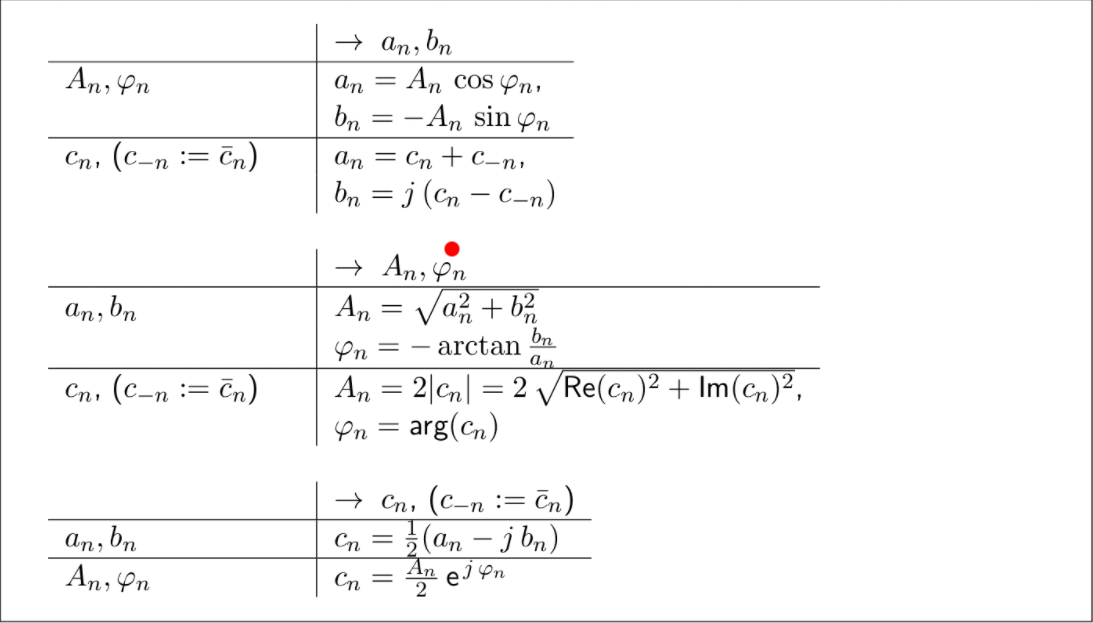
\includegraphics[height=6cm]{Pictures/Umformung.png} \\

  \noindent \textbf{Bedingungen für die Transformation:} 
  \begin{itemize}
  \item Die Funktion muss periodisch sein.
  \item  Innerhalb einer Periode aufteilbar in endlich viele stetige Teilstücke.
  \item Es dürfen keine divergierende Sprungstellen auftauchen.
  \end{itemize}

  \subsubsection{CTFT (analoge, nicht-periodische Signale)}
  \label{sec:sub:sub:ctft}

  \noindent Der Sinn der CTFT: Man möchte vom Zeitsignal $x(t)$ zum Frequenzspektrum $X(\omega)$. \\
  \noindent Die Idee der CTFT: Man nimmt die Fourierreihe und lässt $T_p \to \infty$ gehen: \\
  \begin{equation}
    \label{eq:4}
      \begin{split}
      X(\omega) &= \int_{-\infty}^{ \infty} x(t) \cdot e^{-j \omega t}\ d t\ (CTFT/FT) \ (aus\ 5) \\
      x(t) &= \frac{1}{2\pi} \int_{-\infty}^{ \infty} X(\omega) \cdot e^{j \omega t}\ d \omega\ (ICTFT/IFT) \ (aus\ 6) 
      \end{split}
    \end{equation}

 \noindent   Herleitung:\\
  \noindent Wir definieren eine Hilfsvariable: $\omega_n = n\omega_p$, sodass gilt:
  $\omega_{n+1} - \omega_n = \omega_p = \frac{2\pi}{T_p}$ und beginnen mit:
  $$x(t) = \sum_{n=-\infty}^{\infty} c_n e^{j \omega_n t}$$
  und
  $$c_n := \frac{1}{T_p}\int_{-\frac{T_p}{2}}^{\frac{T_p}{2}}x(t) \cdot e^{-j \omega_n t}\ dt$$

  \noindent Wir definieren eine Funktion in Abhängigkeit von $\omega_n$:
  
  \begin{equation}
  \label{eq:5}
    \begin{split}
    X(\omega_n) &:= \frac{2\pi}{\omega_p}c_n\ \ \big( \Leftrightarrow c_n = \frac{\omega_p}{2\pi}X(\omega_n)\big)\\
    &= \int_{-\frac{T_p}{2}}^{\frac{T_p}{2}}x(t) \cdot e^{-j \omega_n t}\ d t
    \end{split}
  \end{equation}

  \noindent Das neu gewonnene $c_n$ wird nun als Koeffizient in die ursprüngliche komplexe Fourierreihe eingesetzt:

  \begin{equation}
    \label{eq:6}
      \begin{split}
      x(t) &= \sum_{n=-\infty}^{\infty}\frac{\omega_p}{2\pi}X(\omega_n)e^{j\omega_n t}\\
      &= \frac{1}{2\pi} \sum_{n=-\infty}^{\infty} X(\omega_n) e^{j\omega_n t} \omega_p \\
      &= \frac{1}{2\pi} \sum_{n=-\infty}^{\infty} X(\omega_n) e^{j\omega_n t} \ (\omega_{n + 1} - \omega_n)  \\
      \end{split}
    \end{equation}

    \noindent Lässt man nun $T_p \to \infty$ gehen, wird $\omega_p$ immer kleiner und die Unterteilungen $\omega_n$ wandern dichter zueinander
    und im Grenzfall ein kontinuierlicher Verlauf $(\omega_ n \to \omega)$ und man erhält ein Riemann-Integral. Daraus folgert sich die oben aufgeführten Integrale für $x(t)$ und $X(\omega)$.\\

    \noindent  \textbf{Bemerkungen:}
    \begin{itemize}
      \item Stärke des Vorhandenseins einer Frequenz: $|X(\omega)|$
      \item Verschiebung der einzelenen Frequenzen: $\varphi = \arg(X(\omega))$
      \item Es gilt: $\overline{X(\omega)} = X(-\omega)$
      \item Bei reellen Signalen ist Betragsspektrum $|X(\omega)|$ symmetrich um Null
    \end{itemize}

    \subsubsection{Einschub: Die kontinuierliche Faltung}
  \label{sec:sub:sub:faltung}

    
  \begin{equation}
    \label{eq:7}
      \begin{split}
      y(t) &:= x_1 (t) * x_2 (t) = \int_{-\infty}^{\infty} x_1 (\tau) \cdot x_2 (t-\tau)\ d \tau \\
      \end{split}
    \end{equation}
  
    \noindent (Integral)\\
    \noindent Mit der Laufvariable $\tau$ läuft man $x_1$ forwärts durch und $x_2$ rückwärts aber um $t$ verschoben durch. \\
    $t$ ist hier als fester, bekannter Wert zu interpretieren. \\

    \noindent(Faltung) (Man macht das was oben drüber steht für jedes beliebige $t$)\\
    \noindent Man legt ein $\tau$ für $x_1$ und $x_2$ fest, verändert $t$ laufend und sieht sich die Schnittfläche der beiden Funktionen an. \\

    \noindent Main Purpose in der Signalverarbeitung: Abschwächung / Auslöschung von hohen Frequenzen.

  \subsubsection{Einschub: Der Delta-Impuls}
  \label{sec:sub:sub:delta-impuls}

  \noindent Wir definieren eine Funktion:
  \begin{equation}
    \label{eq:8}
    \begin{split}
    \delta (t) &= 0\ \ for\ t \neq 0 \\    
    \int_{-\infty}^{\infty} \delta (t)\ d t &= 1
    \end{split}
    \end{equation}
  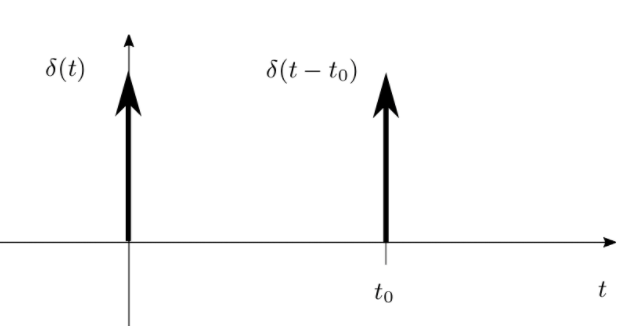
\includegraphics[height=4cm]{Pictures/DeltaImpuls.png} \\

  \noindent  \textbf{Verwendung des Delta-Impulses (Ausblendeigenschaft):}
  \begin{equation}
    \label{eq:9}
    \begin{split}
    \int_{-\infty}^{\infty} x(t) \cdot \delta(t-t_0)\ d t &= \int_{-\infty}^{\infty} x(t_0) \cdot \delta (t-t_0)\ d t \\    
    &= x(t_0) \cdot \int_{-\infty}^{\infty} \delta (t-t_0)\ dt \\
    &=x(t_0)
    \end{split}
    \end{equation}

    \noindent $x(t)$ wird überall ignoriert ausser an der Stelle an der $\delta(t-t_0) \neq 0$, d.h. bei $t = t_0$.\\
    Quasi eine Abtastung der Funktion $x(t)$ an Stelle $t_0$.\\

    \noindent \textbf{Fouriertransformation des Delta-Impulses:}
    $$\int_{-\infty}^{\infty} \delta(t) \cdot e^{-j\omega t}\ dt = \int_{-\infty}^{\infty} \delta(t) \cdot e^{-j\omega 0}\ dt = \int_{-\infty}^{\infty} \delta(t) = 1$$
    $$\delta(t) \TransformHoriz 1 $$ 
    Das Spektrum des Delta-Impulses enthält alle Frequenz mit Gewicht 1! \\

    \noindent \textbf{Die Stammfunktion des Delta-Impulses: $\varepsilon(t)$:}
    $$\varepsilon (t) = \int_{-\infty}^{t} \delta(\tau)\ d \tau \Leftrightarrow  \frac{d}{dt} \varepsilon (t) = \delta (t) $$\\

     \noindent \textbf{Fouriertransformation der Sprungfunktion:}
     $$\varepsilon(t) \TransformHoriz \pi \cdot \delta(\omega) + \frac{1}{j\omega} $$

  \subsubsection{Faltung mit dem Delta-Impuls}
  \label{sec:sub:sub:faltung-mit-delta-impuls}

  \begin{equation}
    \label{eq:10}
    \begin{split}
    x(t) * \delta(t-t_0) &= \int_{-\infty}^{\infty} x(\tau) \cdot \delta\big((t-t_0) - \tau\big)\ d \tau  \\
    &= \int_{-\infty}^{\infty} x(\tau) \cdot \delta \big(\tau -(t-t_0)\big)\ d \tau \\    
    &=x(t - t_0)
    \end{split}
    \end{equation}

\noindent    Kurz bedeutet das
    $$x(t) * \delta(t-t_0) = x(t-t_0)\ ,$$
    und für $t_0 = 0$
    $$x(t) * \delta(t) = x(t)\ .$$
    \noindent Der Delta-Impuls ist das Neutrale Element bezüglich der Faltung!

  \subsubsection{Besonderheiten der CTFT}
  \label{sec:sub:sub:besonderheiten-ctft}

  \noindent \textbf{Eigenschaften der CTFT:}\\
  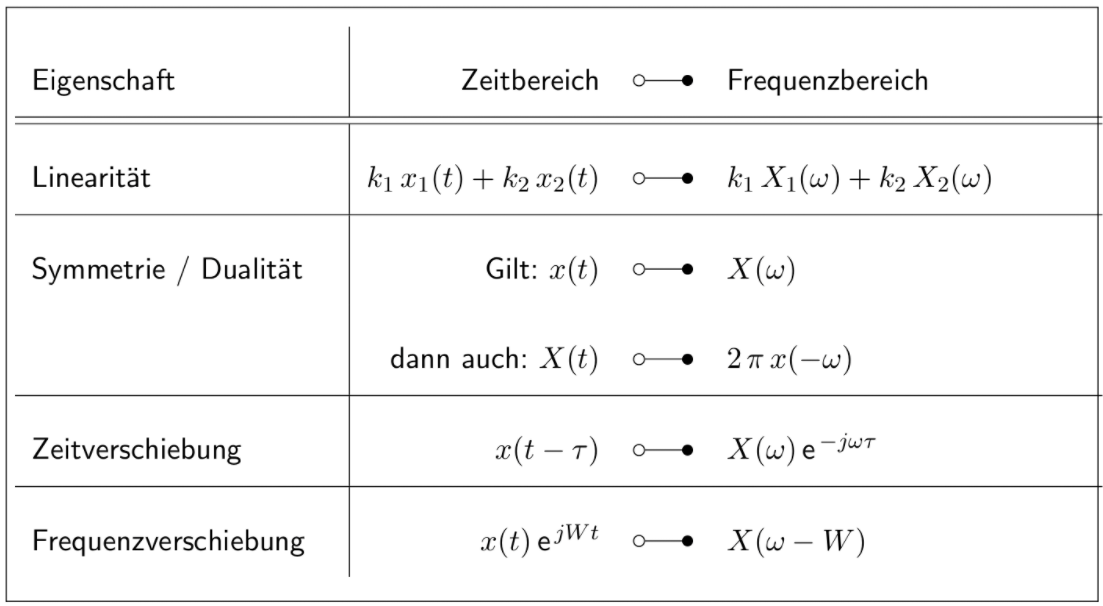
\includegraphics[height = 7cm]{Pictures/EigenschaftenCTFT.png}\\
  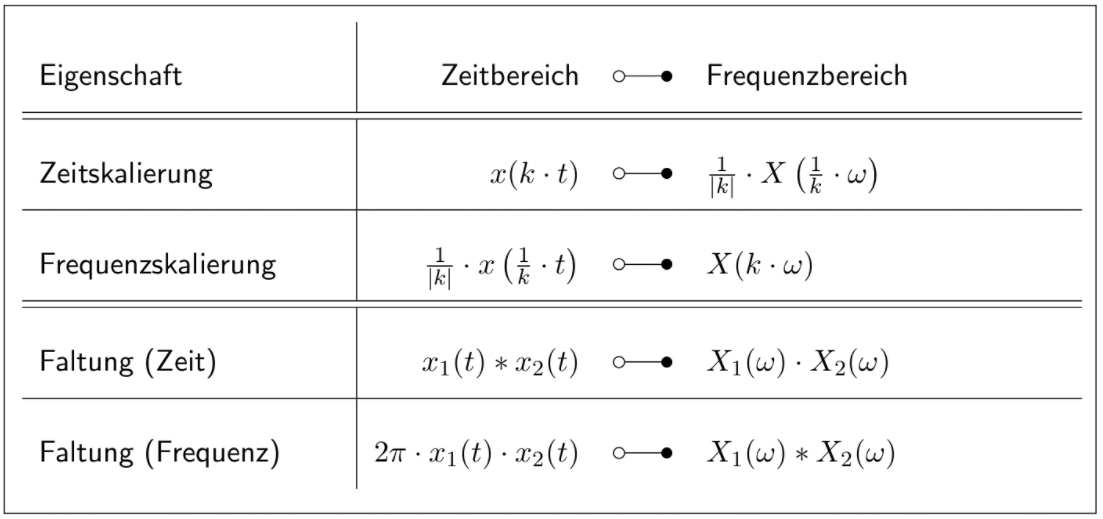
\includegraphics[height = 6cm]{Pictures/EigenschaftenCTFT2.png}\\
  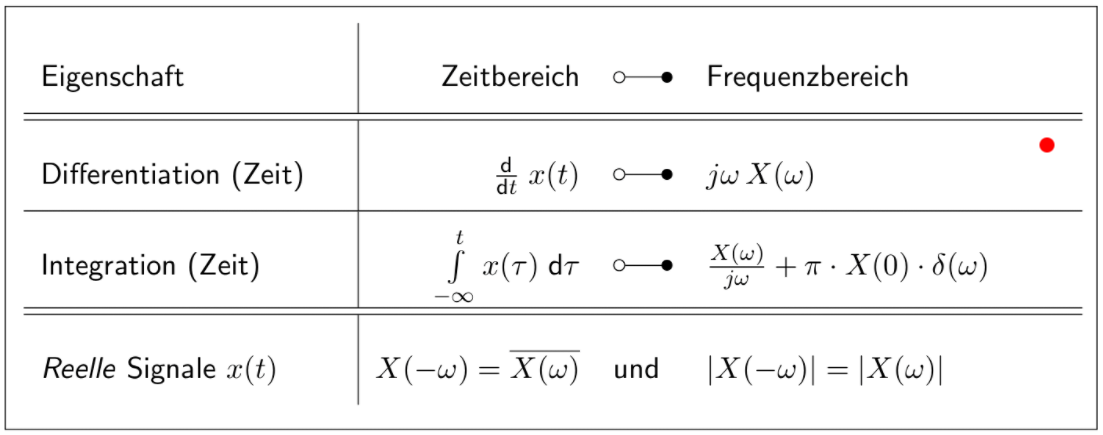
\includegraphics[height = 5cm]{Pictures/EigenschaftenCTFT3.png} \\

  \noindent \textbf{Signaldauer-Bandbreite-Produkt:}\\
  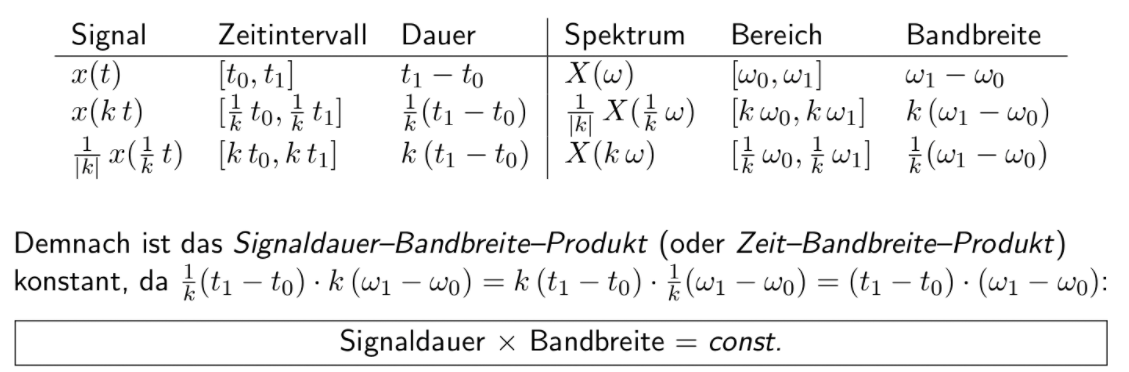
\includegraphics[height=5cm]{Pictures/SignalBand.png} \\

  \noindent \textbf{Korrespondenzen der CTFT:} \\
  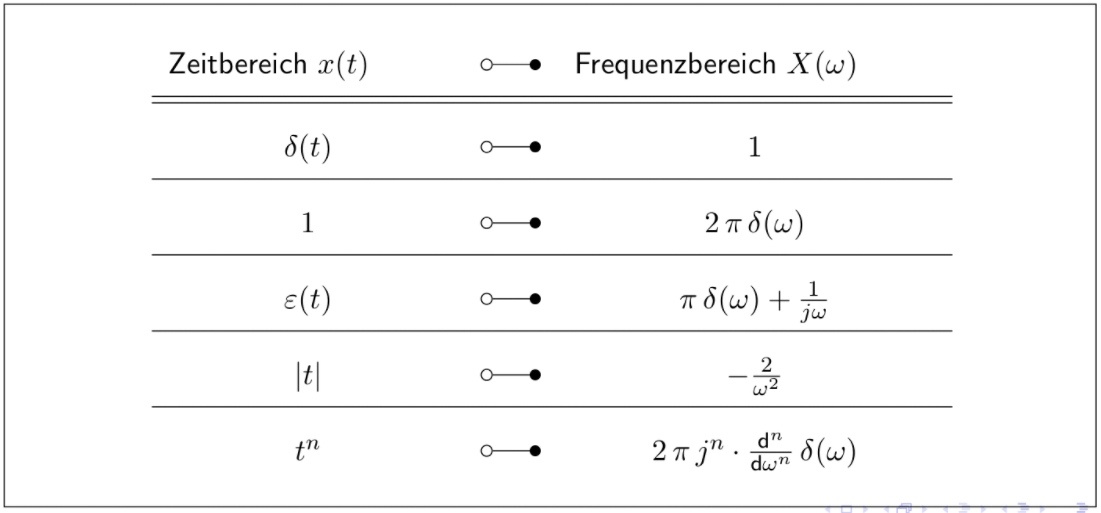
\includegraphics[height = 6cm]{Pictures/Korrespondenz.png}\\
  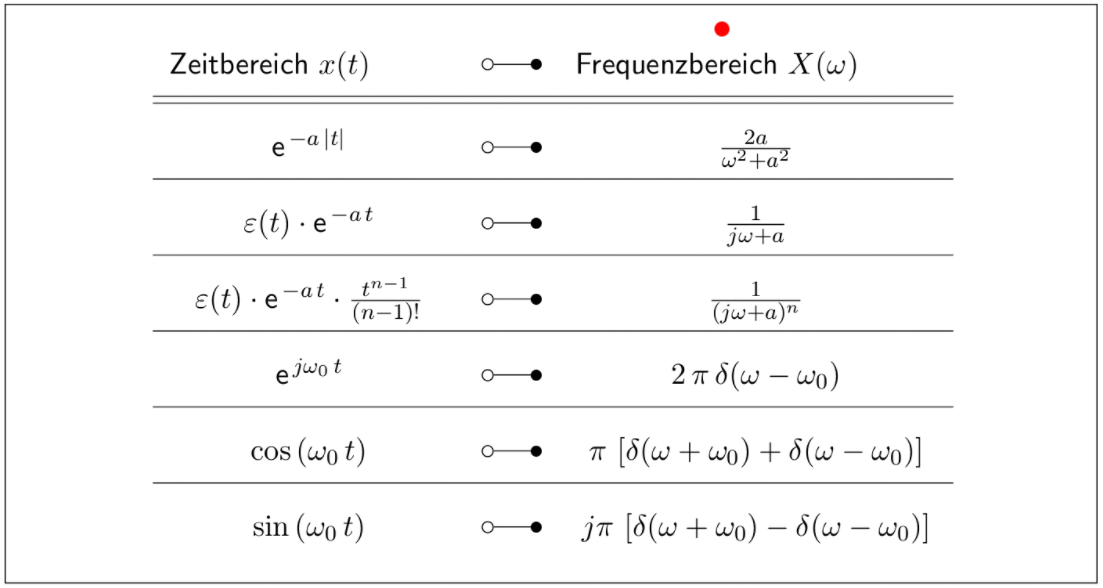
\includegraphics[height = 7cm]{Pictures/Korrespondenz2.png}\\
  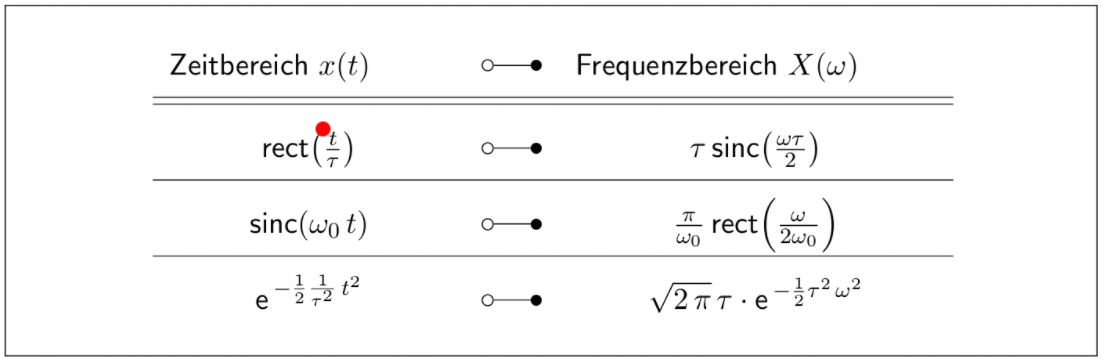
\includegraphics[height = 5cm]{Pictures/Korrespondenz3.png}

  \newpage

  \subsection{Diskrete Signale}
  \label{sec:sub:diskrete-signale}

  \subsubsection{Delta-Kamm}
  \label{sec.sub:sub:delta-kamm}
  \noindent Die Idee eines Delta-Kamms: Aus einer kontinuierlichen Funktion wird eine Zahlenfolge gemacht. \\
  
\noindent Um eine Zahlenfolge aus einer kontinuierlichen Funktion zu erhalten, muss diese abgetastet werden. 
Die Abtastung einer kontinuierlichen Funktion erfolgt mit einem Delta-Kamm:
  \begin{equation}
    \label{eq:11}
      \sum_{n = -\infty}^{\infty} \delta (t-n\Delta T_A)
  \end{equation}

\noindent Der Delta-Kamm stellt eine Schar einzelner Delta-Impulsen an bestimmten gewünschten Abtastungsorten mit gleichem Abstand voneinander dar: \\
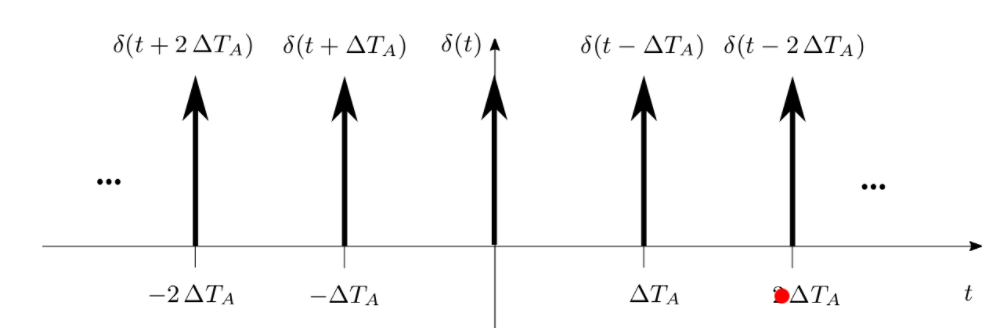
\includegraphics[height=5cm]{Pictures/DeltaKamm.png}

\subsubsection{Abgetastetes Signal}
  \label{sec.sub:sub:abgetastetes-signal}
\noindent Ein abgetastetes Signal ist mit Hilfe des Delta-Kamms definiert durch:
\begin{equation}
  \label{eq:12}
    x_A(t) := x(t) \cdot \sum_{n = -\infty}^{\infty} \delta (t-n\Delta T_A)
\end{equation} 
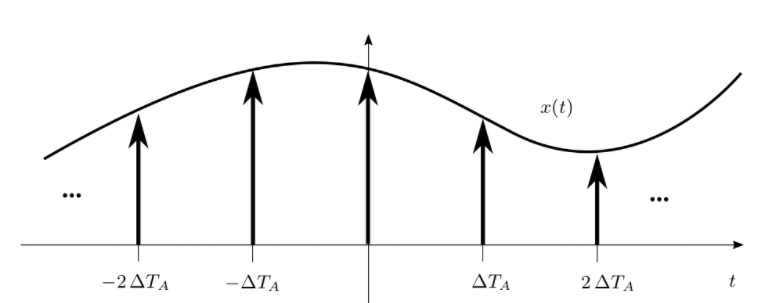
\includegraphics[height=5cm]{Pictures/AbgetastetSignal.png} \\
\noindent $x_A(t)$ wird auch als Diskretes Signal bezeichnet.

\subsubsection{DTFT (diskrete, nicht-periodische Signale)}
  \label{sec.sub:sub:dtft}

  \noindent Mit Hilfe der Ausblendeigenschaft des Delta-Impulses kann man die Fouriertransformation eines solchen abgetasteten Signals bestimmen:
  \begin{equation}
    \label{eq:13}
    \begin{split}
      X_A(\omega) &=  \int_{-\infty}^{\infty} x_A(t) \cdot e^{-j \omega t}\ d t \\
      &=  \int_{-\infty}^{\infty} x(t) \cdot \sum_{n = -\infty}^{\infty} \delta (t-n\Delta T_A) e^{-j \omega t}\ d t\\
      &= \sum_{n = -\infty}^{\infty} \int_{-\infty}^{\infty} x(t) e^{-j\omega t} \cdot \delta(t-n\Delta T_A)\ dt\\
      &= \sum_{n=-\infty}^{\infty} x(n\Delta T_A) e^{-j\omega n \Delta T_A}
    \end{split}
  \end{equation} 
  \\
  \noindent  \textbf{Bemerkungen:}
  \begin{itemize}
    \item Ein diskretes Zeitsignal führt dennoch zu einem kontinuierlichen Frequenzspektrum
    \item Durch Abtastung eines Zeitsignals mit Zeitabständen $\Delta T_A$ wird Frequenzspektrum periodisch mit Periodendauer $\omega_p:= \frac{2\pi}{\Delta T_A}$
    \item diskretes Zeitsignal $\TransformHoriz$ periodisches Spektrum
    \item periodisches Zeitsignal $\TransformHoriz$ diskretes Spektrum
    \item Zusammenhang CTFT und DTFT: $x_A(\omega) = \frac{1}{\Delta T_A} \sum_{ =-\infty}^{\infty} X\Big(\omega - \frac{2\pi n}{\Delta T_A}\Big)$
  \end{itemize}

  \subsubsection{Abtasttheorem}
  \label{sec.sub:sub:abtasttheorem}

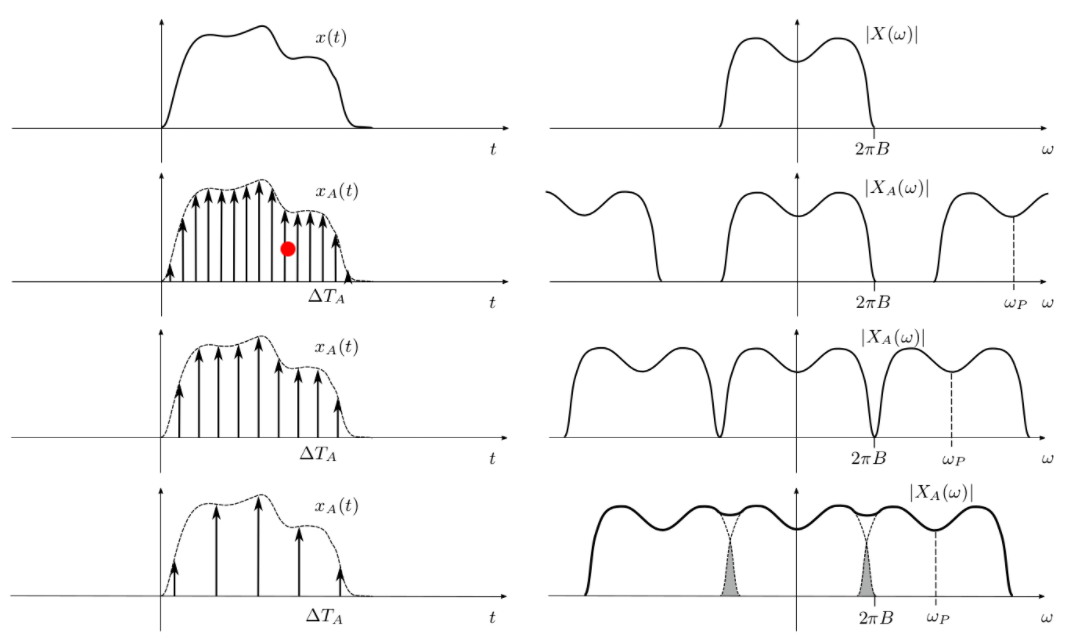
\includegraphics[height=9cm]{Pictures/Abtasttheorem.png} \\
\noindent Man folgert: $\omega_P > 2 \cdot 2\pi B$

\noindent Daraus ergibt sich das eigentliche Abtasttheorem:
\begin{equation}
  \label{eq:14}
  \begin{split}
    f_A = \frac{1}{\Delta T_A} > 2 \cdot B
    \Rightarrow \Delta T_A < \frac{1}{2 \cdot B}
  \end{split}
\end{equation} 

\noindent Ist das Abtasttheorem beim Abtasten eines Signales eingehalten, so kann versichert werden,
dass keine Informationen des Originalsignals verloren gehen und eine Rekonstruktion ist möglich.\\
$\Rightarrow$ "Mindestens mit der doppelt so grossen Frequenz wie im Originalsignal vorhanden ist abtasten." \\

\noindent  \textbf{Bemerkungen:}
  \begin{itemize}
    \item Die höchsten Frequenzen sind die, die zuerst unter der Verletzung des Abtasttheorems leiden (Unterabtastung)
    \item Informationsverlust ist nicht leicht zu beheben
    \item In der Praxis verwendet man häufig eine deutliche Überabtastung \\
  \end{itemize}

  \subsubsection{Rekonstruktion von abgetasteten Signalen}
  \label{sec.sub:sub:rekonstruktion-von-abgetasteten-signalen}

  \noindent   Unter der Annahme, dass das Abtasttheorem mit Zeitintervallen $\Delta T_A$ nicht verletzt wird,
  kann aus den diskreten Abtastwerten $x(n \Delta T_A)$ 
  die kontinuierliche Originalfunktion $x(t)$ rekonstruiert werden mit:
  \begin{equation}
    \label{eq:15}
    \begin{split}
     x(t) &:= \sum_{n=-\infty}^{\infty} x(n \Delta T_A) \cdot sinc\Big(\frac{\pi}{\Delta T_A}(t-n\Delta T_A)\Big)
    \end{split}
  \end{equation} 
  $\Rightarrow$ "Man interpoliert die diskreten Punkten mit der $sinc$-Funktion." \\

  \noindent Herleitung: \\
  \noindent 1. Schritt: Isolieren einer Periode durch Fenstern\\
  Man verwendet einen wichtigen Trick: Das sogenannte Fenstern von Signalen. \\
  Man multipliziert die periodische Fouriertransformierte des Abtastsignals $X_A(\omega)$ 
  mit einem Rechteckpuls der Breite $\omega_P$, 
  um die Fouriertransformierte des Originalsignals $X(\omega)$ zurück zu gewinnen:\\
  
  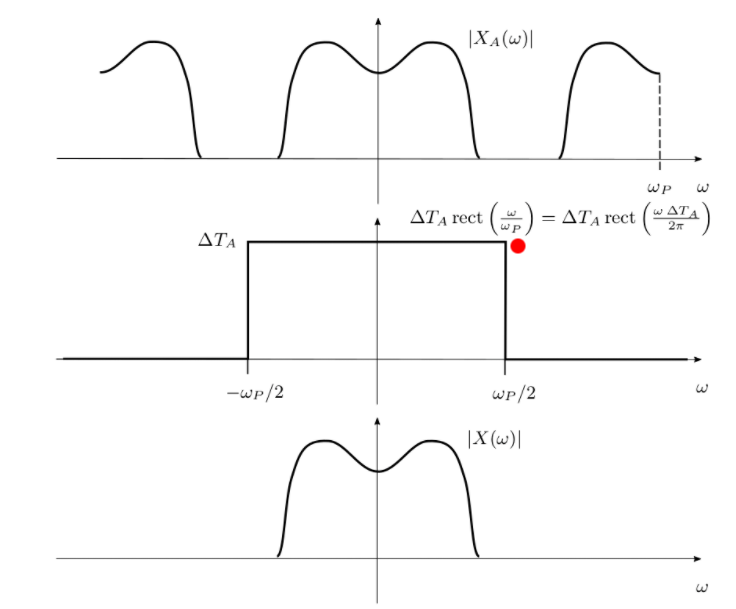
\includegraphics[height = 12cm]{Pictures/Fenstern.png}

  \noindent Signal Fenstern mathematisch: \\
  \begin{equation}
    \label{eq:116}
    \begin{split}
      X(\omega) &= X_A(\omega) \cdot \Delta T_A \cdot rect\Big(\frac{\omega}{\omega_P}\Big) \\
      &= X_A(\omega) \cdot \Delta T_A \cdot rect\Big(\frac{\omega \Delta T_A}{2\pi}\Big)
    \end{split}
  \end{equation} 

  \noindent 2. Schritt: Zurücktransformieren\\
  (Multiplikation im Spektrum $\Rightarrow$ Faltung im Zeitsignal)
  \begin{equation}
    \label{eq:17}
    \begin{split}
      X(\omega) &\TransformHoriz x_A(t) * sinc(\frac{t\pi}{\Delta T_A}) \\
        &= \int_{-\infty}^{\infty}x(\tau) \cdot \sum_{n=-\infty}^{\infty} \delta(\tau - n\Delta T_A) \cdot sinc\Big(\frac{\pi}{\Delta T_A}(t-\tau)\Big)\ d\tau \\
         &= \sum_{n=-\infty}^{\infty} \int_{-\infty}^{\infty}x(\tau) \cdot sinc\Big(\frac{\pi}{\Delta T_A}(t-\tau)\Big) \delta(\tau - n\Delta T_A)\ dt \tau \\
         &= \sum_{n=-\infty}^{\infty} x(n \Delta T_A) \cdot sinc\Big(\frac{\pi}{\Delta T_A}(t-n\Delta T_A)\Big) = x(t) 
        \end{split}
  \end{equation} 






















\end{document}